\section{Complexity Analysis via Symbolic Execution Schemes}
\label{sec:symbolic}

Our approach to complexity analysis is based on a semi-automatic procedure involving symbolic evaluation.
In the previous section we presented formulae to compositionally estimate the complexity factors for
\emph{non-leaf states} of operational semantics under assumption that coresponding estimations for
\emph{leaf states} are given. In order to obtain corresponding estimations for relations as whole we
would need to take into account the effects of relational invocations, including the recursive ones.

Another observation is that as a rule we are interested in complexity estimations in terms of some \emph{metatheory}. For
example, dealing with relations on lists we would be interested in estimations in terms of list lengths,
with trees~--- in terms of depth or number of nodes, with numbers~--- in terms of their values, etc. It is
unlikely that a generic term-based framework would provide such a specific information automatically. Thus,
a viable approach would be to extract some inequalities involving the complexity factors of certain relational
calls automatically and then let a human being solve these inequalities in terms of a relevant metatheory.
In the section we present 

For the sake of clarity we will provide a demonstration of complexity analysis for a specific example~---
\lstinline|append$^o$| relation from the introduction~--- throughout the section.

The extraction procedure utilizes symbolic execution technique and is completely automatic.
It turns out that the semantics we have is already abstract enough to be used for symblolic
execution with minor adjustments.
In this symbolic procedure we mark some of the logic variables as ``grounded'' and at certain
moments substitute them with ground terms.
Informally, for some goal with some free logic variables we consider the complexity of a search
procedure which finds the bindings for all non-grounded variables based on the ground values
substituted for the grounded ones.
This seach procedure is defined precisely by the operational semantics; however, as the concrete
values of grounded variables are unknown (only the fact of their \emph{groundness}), the whole
procedure becomes symbolic.
In particular, in unification the groundness can be propagated to some non-grounded free variables.
Thus, the symbolic execution is determined by a set of grounded varibles (hereafter denoted
as $V\subset\mathcal A$). The initial choice of $V$ determines the problem we analyze.

In our example the objective is to study the execution when we specialize the first two arguments with
ground values and left the last argument free. Thus, we start with the goal \lstinline|append$^o$ $a$ $b$ $ab$|
(where $a$, $b$ and $ab$ are distinct free logic variables) and set the initial $V = \{ a, b \}$.

We can make an important observation that both complexity factors ($d$ and $t$) are stable w.r.t. the renaming of
free variables; moreover, they are also stable w.r.t. the change of the fresh variables counter as long as it stays
adequate, and change of current substitution, as long as it gives the same terms after application.
Formally, the following lemma holds:

\begin{replemma}{lem:measures_changing_env}
Let $s = \taskst{g}{\mkenv{\sigma}{n}}$ and $s' = \taskst{g^\prime}{\mkenv{\sigma^\prime}{n^\prime}}$ be two well-formed states.
If  there exists a bijective substitution $\pi \colon FV\,(g \sigma) \to FV\,(g^\prime \sigma^\prime)$ such that
$g \sigma \pi = g^\prime \sigma^\prime $, then $d\,(s) = d\,(s^\prime)$ and $t\,(s) = t\,(s^\prime)$.
\end{replemma}

The lemma shows that the set of states in which a call to relation has to be analyzed can
be narrowed down to a certain family of states. 

\begin{definition} Let $g$ be a goal. An initial state for $g$ is $init\,(g)=\taskst{g}{(\varepsilon, \ninit\,(g))} $
with $ n_{init}\,(g) = \min\, \{ n \mid FV\,(g) \subseteq \{ \alpha_1\dots\alpha_n \} \} $
\end{definition}

Due to the Lemma~\ref{lem:measures_changing_env} it is sufficient to consider only the family of initial states since an arbitrary state
encountered throughout the execution can be transformed into an initial one while preserving both the semantics and
complexity factors. Thus, the analysis can be performed in a compositional manner where each call can be analyzed separately.
For our example the family of initial states $q^{appn}(\mathbf{a}, \mathbf{b}) = init\,(\lstinline|append$^o$ $\mathbf{a}$ $\mathbf{b}$ $ab$|)$ for arbitrary ground
terms $\mathbf{a}$ and $\mathbf{b}$.

As we are aiming at the complexity estimation depending on specific ground values substituted for grounded variables, in general case extracted
inequalities have be parameterized by \emph{valuations}~--- mappings from the set of grounded variables to ground terms. As the new variables
are added to this set during the execution, the valuations need to be extended for these new variables. The following definition introduces this notion.

\begin{definition}
  Let $ V \subset U \subset \mathcal{A} $ and $ \rho \colon V \to \mathcal{T}_{\emptyset} $ and $ \rho^\prime \colon U \to \mathcal{T}_{\emptyset} $ be two valuations. We say that $\rho^\prime$ extends $\rho$ (denotation: $ \rho^\prime \succ \rho$) if $\rho^\prime\,(x) = \rho\,(x)$ for all $x \in V$.
\end{definition}

The main objective of the symbolic execution in our case is to find constraints on valuations for every leaf goal in the body of a relation that determine
whether the execution will continue and how a valuation changes after this goal. For internal relational calls we describe constraints in term of denotational
semantics (to be given some meaning in terms of metatheory later). We can do it beacuse of a precise equivalence between the anwers found by operational semantics
and values described by denotational semantics thanks to soundness and completness as well as our requirements of grounding and non-repetitiveness of calls.

Our symbolic treatment of equalities relies on the fact that subtitutions of ground terms commute, in a certain sense, with unifications. More specifically,
we can use the most general unifier for two terms to see how unification goes for two terms with some free variables substituted with ground terms.
The most general unifier may contain bindings for both grounded and non-grounded variables. Potential most general unifier for terms after substitution
contains the same bindings for non-grounding terms (with valuation applied to their rhs), while bindings for grounding variables turn into equations that
should be satisfied by the unifier with ground value on the left and bound term on the right. In particular, this means that all variables in bindings for
grounded variables become grounded, too. We can use this observation to define an iterative process that determines the updated set of grounded
variables $\upd{U}{\delta}$ for a current set $U$ and a most general unifier $\delta$ and a set of equations $\constr{\delta}{U}$ that should be
respected by the valuation.

\[
\begin{array}{rcl}
\upd{U}{\delta} &=& \begin{cases}
                           U & \quad\forall x \in U : FV\,(\delta\,(x)) \subset U \\
                           \upd{U \cup \displaystyle\bigcup\limits_{x \in U} FV\,(\delta\,(x))}{\delta} & \quad\mbox{otherwise}
                          \end{cases}\\
\constr{\delta}{U} &=& \{ x = \delta\,(x) \mid x \in U \cap \mathcal{D}om\,(\delta) \}
\end{array}
\]

Using these definitions we can describe symbolic unification by the following lemma.

\begin{replemma}{lem:symbolic_unification_soundness}
Let $t_1$, $t_2$ be terms,  $V \subset \mathcal{A}$ and $\rho \colon V \to \grterms$ be a valuation. If $mgu\,(t_1, t_2) = \delta$ and $U = \upd{V}{\delta} $  then $t_1 \rho$ and $t_2 \rho$ are unifiable iff there is some $\rho' \colon U \to \grterms$ such that $\rho' \succ \rho$ and $\forall (y = t) \in \constr{\delta}{U}\,:\, t_1 \rho = t_2 \rho'$.
In such case $\rho'$ is unique and $ \rho \circ mgu\,(t_1 \rho, t_2 \rho) = \delta\circ\rho' $ up to alpha-equivalence (e.g. there exists a bijective substitution $\pi : FV(t_1) \to FV(t_2)$, s.t. $ \rho \circ mgu\,(t_1 \rho, t_2 \rho) = \delta \circ\rho'\circ \pi$).
\end{replemma}

In our description of the extraction process we use a visual representation of symbolic execution of relation body for a given set of grounded variables in a form of a \emph{symbolic scheme}.
Symbolic scheme is a tree-like structure with different branches corresponding to execution of different disjuncts and nodes corresponding to equalities and relational calls in the body
augmented with subsets of grounded variables at the point of execution.\footnote{Note the difference with conventional symbolic execution graphs
with different branches representing mutually exclusive paths of evaluation, not the different parts within one evaluation.} Constrains for substituted
grounded variables that determine whether the execution continues are presented as labels on the edges of a scheme.

More formally, each scheme is built as a composition of the following five forms (schemes are indexed by subsets of grounded variables with $\Upsilon = 2^{\mathcal{A}}$ denoting such subsets):

\[
\renewcommand{\arraystretch}{3}
\begin{array}{ccm{0.5cm}m{3cm}m{4cm}m{4cm}}
  \schemewithvset{\mathfrak{S}}{\Upsilon} & = && \schemenode{$\unigoal{\mathcal{T}_\mathcal{A}}{\mathcal{T}_\mathcal{A}}$} & \schemenode{$\invokegoal{R^k}{\mathcal{T}_\mathcal{A}}{\mathcal{T}_\mathcal{A}}$} 
                                       & \multirow{2}{*}{\schemefork{$\schemewithvset{\mathfrak{S}}{\Upsilon}$}{$\schemewithvset{\mathfrak{S}}{\Upsilon}$}} \\
                                   &   && \schemesarrow{$\unigoal{\mathcal{T}_\mathcal{A}}{\mathcal{T}_\mathcal{A}}$}{$\{\mathcal{A}=\mathcal{T}_\mathcal{A}\}$}{$\schemewithvset{\mathfrak{S}}{\Upsilon}$}
                                       & \schemedarrow{$\invokegoal{R^k}{\mathcal{T}_\mathcal{A}}{\mathcal{T}_\mathcal{A}}$}{$(\mathcal{T}_\mathcal{A}, \dots, \mathcal{T}_\mathcal{A}) \in \sembr{R^k}$}{$\schemewithvset{\mathfrak{S}}{\Upsilon}$}
                                       & 
\end{array}
\]

Note, the constrains after nodes of different types differ: unification puts a constraint in a form of a set of equations on substituted ground values that should be respected while
relational call puts a constraint in a form of a tuple of ground terms that should belong to denotational semantics of a relation.

The construction of a scheme for a given goal (initially, the body of a relation) mimics a regular execution of a relational program. The derivation rules for scheme
formation have the following form:

\[ \schemetrans{g}{\Gamma}{\sigma}{n}{V}{\schemewithvset{\mathfrak{S}}{V}} \]

Here $g$ is a goal, $\Gamma$ is a list of \emph{deferred} goals (these goals have to be executed after the execution of $g$ in every branch in the same order,
initially this list is empty; this resembles continuations, but the analogy is not complete), $\sigma$ and $n$ are substitution and counter from current
environment respectively, $V$ is a set of grounded variables at the moment.

\begin{figure}[t]  
\renewcommand{\arraystretch}{3}
  \[
\begin{array}{cr}
  \onepremrule
		{  \schemetrans{g_1}{g_2 : \Gamma}{\sigma}{n}{V}{\schemewithvset{\mathfrak{S}}{V}}  } 
		{  \schemetrans{\conjgoal{g_1}{g_2}}{\Gamma}{\sigma}{n}{V}{ \schemewithvset{\mathfrak{S}}{V} }  } & \ruleno{Conj$_\mathfrak S$}
		\\
                
  % \multicolumn{3}{c}{
  \twopremrule
		{  \schemetrans{g_1}{\Gamma}{\sigma}{n}{V}{\schemewithvset{\mathfrak{S_1}}{V}}  }
		{  \schemetrans{g_2}{\Gamma}{\sigma}{n}{V}{\schemewithvset{\mathfrak{S_2}}{V}}  }
		{  \schemetrans{\disjgoal{g_1}{g_2}}{\Gamma}{\sigma}{n}{V}{\parbox[m]{2cm}{ \schemefork{$\schemewithvset{\mathfrak{S_1}}{V}$}{$\schemewithvset{\mathfrak{S_2}}{V}$}} }  } & \ruleno{Disj$_\mathfrak S$}\\ 
		
		
 \onepremrule
		{  \schemetrans{\substitute{g}{\alpha_n}{x}}{\Gamma}{\sigma}{n + 1}{V}{\schemewithvset{\mathfrak{S}}{V}}  }
		{  \schemetrans{\freshgoal{x}{g}}{\Gamma}{\sigma}{n}{V}{ \schemewithvset{\mathfrak{S}}{V} }  } & \ruleno{Fresh$_\mathfrak S$}\\

 %\multicolumn{3}{c}{
  \schemetrans{\unigoal{t_1}{t_2}}{\epsilon}{\sigma}{n}{V}{\parbox[m]{2cm}{\schemenode{$\unigoal{t_1 \sigma}{t_2 \sigma}$}}}& \ruleno{UnifyLeaf$_\mathfrak S$}\\

 %\multicolumn{3}{c}{
 \schemetrans{\invokegoal{R^k}{t_1}{t_k}}{\epsilon}{\sigma}{n}{V}{\parbox[m]{2cm}{\schemenode{$\invokegoal{R^k}{t_1 \sigma}{t_k \sigma}$}}}& \ruleno{InvokeLeaf$_\mathfrak S$}\\ 
		
 %\multicolumn{3}{c}{
  \onepremrule
		{  \nexists mgu\,(t_1 \sigma, t_2 \sigma)  }
		{  \schemetrans{\unigoal{t_1}{t_2}}{g : \Gamma}{\sigma}{n}{V}{\parbox[m]{2cm}{\schemenode{$\unigoal{t_1 \sigma}{t_2 \sigma}$}}} }& \ruleno{UnifyFail$_\mathfrak S$}\\

 %\multicolumn{3}{c}{
  \threepremrule
		{  mgu\,(t_1 \sigma, t_2 \sigma) = \delta  }
		{  U = \upd{V}{\delta}  }
		{  \schemetrans{g}{\Gamma}{\sigma \delta}{n}{U}{\schemewithvset{\mathfrak{S}}{U}}  }
		{  \schemetrans{\unigoal{t_1}{t_2}}{g : \Gamma}{\sigma}{n}{V}{\parbox[m]{2cm}{\schemesarrow{$\unigoal{t_1 \sigma}{t_2 \sigma}$}{$\constr{\delta}{U}$}{$\schemewithvset{\mathfrak{S}}{U}$}} }   } & \ruleno{UnifySuccess$_\mathfrak S$}\\
		
 %\multicolumn{3}{c}{
  \twopremrule
		{  \mbox{\phantom{XXXXXX}} U =  V \cup \displaystyle\bigcup\limits_{i} FV\,(t_i \sigma) }
		{  \schemetrans{g}{\Gamma}{\sigma}{n}{U}{\schemewithvset{\mathfrak{S}}{U}} \mbox{\phantom{XXXXXX}} }
		{  \schemetrans{\invokegoal{R^k}{t_1}{t_k}}{g : \Gamma}{\sigma}{n}{V}{ \parbox[m]{2cm}{\schemedarrow{$\invokegoal{R^k}{t_1 \sigma}{t_k \sigma}$}{$ (t_1 \sigma, \dots, t_k \sigma) \in \sembr{R^k} $}{$\schemewithvset{\mathfrak{S}}{U}$}} }   } & \ruleno{Invoke$_\mathfrak S$}
 \end{array}
\]
\caption{Scheme Formation Rules}
\label{fig:scheme_formation}
\end{figure}

The rules are shown in \figureword~\ref{fig:scheme_formation}. \ruleno{Conj$_\mathfrak S$} and \ruleno{Disj$_\mathfrak S$} are structural rules: when investigating conjunctions we defer
the second conjunct by adding it to $\Gamma$ and continue with the first conjunct; disjunctions simply result in forks. \ruleno{Fresh$_\mathfrak S$} introduces a fresh logic
variable (not grounded) and updates the counter of occupied variables. When investigated goal is equality or relational call it is added as a node to the scheme. If there are
no deferred goals, then this node is a leaf (rules \ruleno{UnifyLeaf$_\mathfrak S$} and \ruleno{InvokeLeaf$_\mathfrak S$}). Equality is also added as a leaf if there are some deferred goals,
but the terms are non-unifiable and so the execution stops (rule \ruleno{UnifyFail$_\mathfrak S$}). If the terms in the equality are unifiable and there are deferred goals
(rule \ruleno{UnifySuccess$_\mathfrak S$}), the equality is added as a node and the execution continues for the deferred goals, starting from the leftmost one; also the set of grounded variables
is updated and constraint labels are added for the edge according to \lemmaword~\ref{lem:symbolic_unification_soundness}. The same true for relational calls: if there are some deferred goals
(rule \ruleno{Invoke$_\mathfrak S$}), all variables occurring in a call become grounded (due to the grounding condition we imposed) and should satisfy the denotational semantics
of the invoked relation.

\begin{figure}[t]
\begin{center}
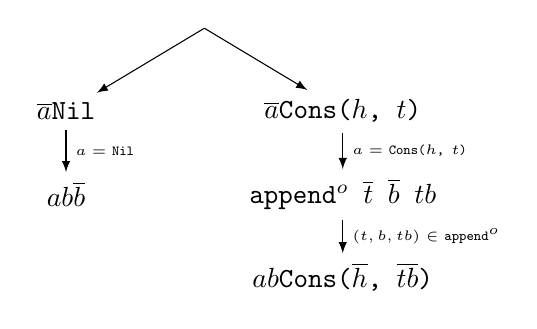
\begin{tikzpicture}[level distance=30pt, sibling distance=10em, edge from parent/.style={draw,-latex}]
   \coordinate   
      child { node {$\unigoal{\overline{a}}{\texttt{Nil}}$}
        child { node {$\unigoal{ab}{\overline{b}}$}
                  edge from parent node[right]{\tiny{${a} = \texttt{Nil}$}} } }
      child { node {$\unigoal{\overline{a}}{\texttt{Cons($h$, $t$)}}$} 
      	child { node {\texttt{append$^o$ $\overline{t}$ $\overline{b}$ $tb$}}
      	   child { node {$\unigoal{ab}{\texttt{Cons($\overline{h}$, $\overline{tb}$)}}$}
      	             edge from parent node[right]{\tiny{$({t}, {b}, {tb}) \in \llbracket \texttt{append$^o$} \rrbracket$}}  }
      	   edge from parent node[right]{\tiny{${a} = \texttt{Cons(${h}$, ${t}$)}$}}  } } ;
\end{tikzpicture}
\end{center}

\caption{Symbolic execution scheme for the goal  \lstinline|append$^o$ $\,a\;$ $b\;$ $ab$|  with initial set of grounded variables $V = \{ a, b \}$. For each node, variables that
  are grounded at the point of execution of this node are overlined. }
\label{fig:example_scheme}
\end{figure}

The scheme constructed by these rules for our \lstinline|append$^o$| example is shown in \figureword~\ref{fig:example_scheme}. For simplicity we do not show the set of grounded
variables for each node, but instead overline grounded variables in-place. Note, all variables that occur in constraints on the edges are grounded after parent node execution.

Now, we can use schemes to see how the information for leaf goals in relation body are combined with conjunctions and disjuntions. Then we can apply formulae
from \sectionword~\ref{sec:scheduling} to get recursive inequalities (providing lower and upper bounds simultaniously) for both complexity factors.

\begin{figure}[t]
\[
\begin{array}{rclcl}
 \mathcal{\nicefrac{D}{T}}\,(&\parbox[m]{1.3cm}{\schemenode{$\unigoal{t_2}{t_2}$}}&)(\rho) &=& 1  \\

 \mathcal{\nicefrac{D}{T}}\,(&\parbox[m]{2.5cm}{\schemenode{$\invokegoal{R^k}{t_1}{t_k}$}}&)(\rho) &=& \nicefrac{d}{t}\,(init\,(\invokegoal{R^k}{t_1 \rho}{t_k \rho})) \\

 \mathcal{\nicefrac{D}{T}}\,(&\parbox[m]{2cm}{\schemesarrow{$\unigoal{t_1}{t_2}$}{$Cs$}{$\schemewithvset{\mathfrak{S}}{U}$}} &)(\rho) &=& 1 +
      \smashoperator{\sum\limits_{\substack{ \rho' \colon V \to \grterms \\
                                      \rho' \succ \rho \\
                                      \forall (y, t) \in Cs\,:\, \rho'\,(y) = t\, \rho'  }}}
           \mathcal{\nicefrac{D}{T}}\,(\schemewithvset{\mathfrak{S}}{U})(\rho')  \\

 \mathcal{\nicefrac{D}{T}}\,(& \parbox[m]{4cm}{\schemedarrow{$\invokegoal{R^k}{t_1}{t_k}$}{ $(t_1, \dots, t_k) \in \sembr{R^k}  $}{$\schemewithvset{\mathfrak{S}}{U}$}} &)(\rho) &=&
      \nicefrac{d}{t}\,(init\,(\invokegoal{R^k}{t_1 \rho}{t_k \rho})) +
      \smashoperator{\sum\limits_{\substack{ \rho' \colon V \to \grterms \\
                                      \rho' \succ \rho \\
                                      (t_1 \rho', \dots, t_k \rho') \in \sembr{R^k}  }}}
           \mathcal{\nicefrac{D}{T}}\,(\schemewithvset{\mathfrak{S}}{U})(\rho')  \\

 \mathcal{\nicefrac{D}{T}}\,(&\parbox[m]{2.5cm}{\schemefork{$\schemewithvset{\mathfrak{S}_1}{V}$}{$\schemewithvset{\mathfrak{S}_2}{V}$}}&)(\rho) &=&
 \mathcal{\nicefrac{D}{T}}\,(\schemewithvset{\mathfrak{S}_1}{V})(\rho) + \mathcal{\nicefrac{D}{T}}\,(\schemewithvset{\mathfrak{S}_2}{V})(\rho)
\end{array}
\]
\caption{Complexity Factors Extraction: $\mathcal D$ and $\mathcal T$}
\label{fig:scheduling_extraction_d_t}
\end{figure}

In this inequalities we need to sum up the values of $d$- and $t$-factor for all leaf goals of a body and for all environments these goals are evaluated for. The leaf goals are
the nodes of the scheme and evaluated environments can be derived from the constraints attached to the edges. So, for this summation we introduce the following notions: $\mathcal{D}$
is the sum of $d$-factor values and $\mathcal{T}$ is the sum of $t$-factor values for execution of the body with specific valuation $\rho$. Their defintions are shown in
the \figureword~\ref{fig:scheduling_extraction_d_t} (both formulas are given in the same figure as the defintions coincide modulo factor denotations). For nodes we take
corresponding value (for equality it always equals to $1$). When going through an equality we sum up the rest with an updated valuation (by \lemmaword~\ref{lem:symbolic_unification_soundness}
this sum always has one or zero summands depending on whether the unification succeeds or not). When going through a relational call we take a sum of all valuations that satisfy the
denotational semantics (these valuations will correspond exactly to the set of all answers produced by the call since operational semantics is sound and complete w.r.t. the denotational
one and because we require all calls to be non-repetitive). For disjunctions we take the sum of both branches.

\begin{figure}[t]
\colorbox{yellow!20}{\parbox{\textwidth}{\textbf{Maybe move this to appendix and leave here the informal description only}}}

\[
\begin{array}{rclcl}
 \mathcal{L}\,(&\parbox[m]{1.3cm}{\schemenode{$\unigoal{t_2}{t_2}$}}&)(\rho) &=& \{init\,(\unigoal{t_2}{t_2})\} \\

 \mathcal{L}\,(&\parbox[m]{2.5cm}{\schemenode{$\invokegoal{R^k}{t_1}{t_k}$}}&)(\rho) &=& \{init\,(\invokegoal{R^k}{t_1 \rho}{t_k \rho})\} \\

 \mathcal{L}\,(&\parbox[m]{2cm}{\schemesarrow{$\unigoal{t_1}{t_2}$}{$Cs$}{$\schemewithvset{\mathfrak{S}}{U}$}} &)(\rho) &=&  \{init\,(\unigoal{t_2}{t_2})\} \cup
      \smashoperator{\bigcup\limits_{\substack{ \rho' \colon V \to \grterms \\
                                      \rho' \succ \rho \\
                                      \forall (y, t) \in Cs\,:\, \rho'\,(y) = t\, \rho'  }}}
           \mathcal{L}\,(\schemewithvset{\mathfrak{S}}{U})(\rho')  \\

 \mathcal{L}\,(& \parbox[m]{4cm}{\schemedarrow{$\invokegoal{R^k}{t_1}{t_k}$}{ $(t_1, \dots, t_k) \in \sembr{R^k}  $}{$\schemewithvset{\mathfrak{S}}{U}$}} &)(\rho) &=&
      \{init\,(\invokegoal{R^k}{t_1 \rho}{t_k \rho})\} \cup
      \smashoperator{\bigcup\limits_{\substack{ \rho' \colon V \to \grterms \\
                                      \rho' \succ \rho \\
                                      (t_1 \rho', \dots, t_k \rho') \in \sembr{R^k}  }}}
           \mathcal{L}\,(\schemewithvset{\mathfrak{S}}{U})(\rho')  \\

 \mathcal{L}\,(&\parbox[m]{2.5cm}{\schemefork{$\schemewithvset{\mathfrak{S}_1}{V}$}{$\schemewithvset{\mathfrak{S}_2}{V}$}}&)(\rho) &=&
 \mathcal{L}\,(\schemewithvset{\mathfrak{S}_1}{V})(\rho) \cup \mathcal{L}\,(\schemewithvset{\mathfrak{S}_2}{V})(\rho)
\end{array}
\]
\caption{Complexity Factors Extraction: $\mathcal L$}
\label{fig:scheduling_extraction_l}
\end{figure}

As we saw in \sectionword~\ref{sec:scheduling} when computing the scheduling factors we need to exclude from the additional cost the value of $d$-factor
for one of the environments (the largest one). This is true for the generalized formula for a whole scheme, too. This time we need to take all executed
environments for all the leaves of a scheme and exclude the $d$-factor value for maximal one (formula for conjunction ensures that we make the exclusion
for the leaf, and the formula for disjunction ensures that we make it for only one of the leaves). So, we will need additional notion $\mathcal{L}$,
similar to $\mathcal{D}$ and $\mathcal{T}$ that will collect all the goals of the form $init\,(g_i \rho)$, where $g_i$ is a leaf goal and $\rho$ is a
valuation corresponding to one of the environments this leaf is evaluated for. The definition of $\mathcal{L}$ is shown in \figureword~\ref{fig:scheduling_extraction_l}.

Now we can formulate the following main theorem that provides the principal recursive approximations, extracted from the scheme for a given goal.

\begin{reptheorem}{extracted_approximations}
Let $g$ be a goal in DNF and all sub-calls encountered during its evaluation are grounding and non-repetitive, and let

\[  \schemetrans{g}{\epsilon}{\varepsilon}{n_{init}(g)}{V}{\schemewithvset{\mathfrak{S}}{V}}  \]

\noindent Then

\[
\begin{array}{rcl}
    d\,(init\,(g\,\rho)) &=& \mathcal{D}\,(\schemewithvset{\mathfrak{S}}{V})(\rho) + \Theta\,(1) \\
   t\,(init\,(g\,\rho)) &=& \mathcal{T}\,(\schemewithvset{\mathfrak{S}}{V})(\rho) + \Theta\,(\mathcal{D}\,(\schemewithvset{\mathfrak{S}}{V})(\rho)
   - \smashoperator{\maxd\limits_{\taskst{g_i}{e_i} \in \mathcal{L}(\schemewithvset{\mathfrak{S}}{V})(\rho)}} d\,(\taskst{g_i}{e_i}) + 1)
\end{array}
\]

\noindent being considered as functions on $\rho \colon V \to T_{\emptyset}$
\end{reptheorem}

The theorem allows us to extract two inequalities (upper and lower bounds) for both factors with a multiplicative constant that is the same for all valuations.

For our example we can extract the following recursive inequalities from the scheme in \figureword~\ref{fig:example_scheme}. For presentation purposes we will
not show valuation in inequalities explicitly, but instead show the ground values of grounded variables (using variables in bold font) that determine each valuation.
\colorbox{yellow!20}{\parbox{\textwidth}{\textbf{For a specific relation this presentation is always easier}}}.

\[
d\,(q^{appn}\,(\mathbf{a}, \mathbf{b}))  = (1 + \sum\limits_{\mathbf{a} = \texttt{Nil}} 1) + (1 + \smashoperator{\sum\limits_{\mathbf{h}, \mathbf{t}: \mathbf{a} = \texttt{Cons($\mathbf{h}$, $\mathbf{t}$)}}} (d\,(q^{appn}\,(\mathbf{t}, \mathbf{b})) + \smashoperator{\sum\limits_{\mathbf{tb} : (\mathbf{t}, \mathbf{b}, \mathbf{tb}) \in \llbracket \texttt{append$^o$} \rrbracket}} 1)) + \Theta\,(1)
\]\\[0.8mm]
\[
\begin{array}{lclc}
t\,(q^{appn}\,(\mathbf{a}, \mathbf{b})) & = & (1 + \sum\limits_{\mathbf{a} = \texttt{Nil}} 1) + (1 + \smashoperator{\sum\limits_{\mathbf{h}, \mathbf{t}: \mathbf{a} = \texttt{Cons($\mathbf{h}$, $\mathbf{t}$)}}} (t\,(q^{appn}\,(\mathbf{t}, \mathbf{b})) + \smashoperator{\sum\limits_{\mathbf{tb} : (\mathbf{t}, \mathbf{b}, \mathbf{tb}) \in \llbracket \texttt{append$^o$} \rrbracket}} 1)) & + \\
 & &\Theta((1 + \sum\limits_{\mathbf{a} = \texttt{Nil}} 1) + (1 + \smashoperator{\sum\limits_{\mathbf{h}, \mathbf{t}: \mathbf{a} = \texttt{Cons($\mathbf{h}$, $\mathbf{t}$)}}} (d\,(q^{appn}\,(\mathbf{t}, \mathbf{b})) + \smashoperator{\sum\limits_{\mathbf{tb} : (\mathbf{t}, \mathbf{b}, \mathbf{tb}) \in \llbracket \texttt{append$^o$} \rrbracket}} 1)) & - \\
& & \smashoperator{\maxd\limits_{\substack{
                                   \mathbf{h}, \mathbf{t}, \mathbf{tb}: \mathbf{a} = \texttt{Cons($\mathbf{h}$, $\mathbf{t}$)} \land \\
                                   (\mathbf{t}, \mathbf{b}, \mathbf{tb}) \in \llbracket \texttt{append$^o$} \rrbracket
                                 }
                                }} \{ d\,(init\,(\unigoal{ab}{\mathbf{b}})), d\,(init\,(\unigoal{ab}{\texttt{Cons($\mathbf{h}$, $\mathbf{tb}$)}})) \} & + 1 
\end{array}
\]


Automatically extracted recursive inequalities as a rule are cumbersome, but they contain all the information on how scheduling affects the complexity.
Often they can be drastically simlified by using a metatheory-level reasoning.

For our example, we are only interested in the case when substituted values represent some lists. We thus pefroms the usual for lists case analysis
considering the first list empty or non-empty. We can also notice that the excluded summand equals to one. So we can rewrite the inequalities in the following way:

\[
\begin{array}{lcl}
d\,(q^{appn}\,(\texttt{Nil}, \mathbf{b})) & = & \Theta\,(1) \\
d\,(q^{appn}\,(\texttt{Cons($\mathbf{h}$, $\mathbf{t}$)}, \mathbf{b})) & = & d\,(q^{appn}\,(\mathbf{t}, \mathbf{b})) + \Theta\,(1) \\
\\
t\,(q^{appn}\,(\texttt{Nil}, \mathbf{b})) & = & \Theta\,(1) \\
t\,(q^{appn}\,(\texttt{Cons($\mathbf{h}$, $\mathbf{t}$)}, \mathbf{b})) & = & t\,(q^{appn}\,(\mathbf{t}, \mathbf{b})) + \Theta\,(d\,(q^{appn}\,(\mathbf{t}, \mathbf{b}))) \\
\end{array}
 \]
 
These trivial linear inequalities can be easily solved:

\[
\begin{array}{lcl}
d\,(q^{appn}\,(\mathbf{a}, \mathbf{b})) & = & \Theta\,(len\,(\mathbf{a})) \\
t\,(q^{appn}\,(\mathbf{a}, \mathbf{b})) & = & \Theta\,(len^2\,(\mathbf{a})) \\
\end{array}
 \]
 
In this case scheduling makes a big difference and changes the asymptotics. Note, we expressed the result using notions from metatheory
($len$ for the length of the list represented by a term).

In contrast, if we consider the conventional definition of \lstinline|append$^o$| the analysis of the call
$q^{appo}\,(\mathbf{a}, \mathbf{b}) = init\,(\texttt{append$^o_{opt}$} \, \mathbf{a} \, \mathbf{b} \, ab)$ is analagous,
but among the candidates for exclusion there is the value $d\,(q^{app}\,(\mathbf{t}, \mathbf{b}))$ since the recursive
call is placed in a leaf. So the last simplified recursive apprioximation is the following (the rest is
the same as in our main example):

\[t\,(q^{appo}\,(\texttt{Cons\,($\mathbf{h}$, $\mathbf{t}$)}, \mathbf{b})) = t\,(q^{appo}\,(\mathbf{t}, \mathbf{b})) + \Theta\,(1) \]

So in this case the complexity of both factors is linear on $len\,(\mathbf{a})$.
